% !TEX encoding = UTF-8 Unicode
\documentclass[12pt]{report}
\usepackage[utf8]{inputenc}
\usepackage{graphicx}
\graphicspath{ {images/} }
% header
\usepackage{fancyhdr}
\pagestyle{fancy}
% bibliography
\usepackage{biblatex}
\addbibresource{references.bib}
% plot
\usepackage{pgfplots}
% code
\def\code#1{\texttt{#1}}
% cource code
\usepackage{listings}
% draft
%\usepackage{draftwatermark}
%\SetWatermarkText{DRAFT}
%\SetWatermarkScale{1}
% link
\usepackage{hyperref}
% flowchart
\usepackage{tikz}
\usetikzlibrary{shapes,arrows}
% color
\usepackage{xcolor}
% from classicthesis
\RequirePackage{booktabs} % for better rules in tables
\RequirePackage{textcase} % for \MakeTextUppercase
\RequirePackage{soul}
% figure position
%\usepackage{float}
% glossary
\usepackage{glossaries}
% 3D plot
\usepgfplotslibrary{patchplots}
\usepackage[pdftex]{ocg}
\usepackage{pgfplots}
\pgfplotsset{compat=newest}
% subfigure
\usepackage{subcaption}
% caption style
\usepackage[font={it}]{caption}
% degree
\usepackage{gensymb}
\usepackage[T1]{fontenc}
\usepackage{textcomp}
\makeglossaries

\newglossaryentry{eCore}{
	name={eCore},%
	description={An Epiphany core}%
}

\newglossaryentry{FPGA}{
	name={FPGA},%
	description={Field-Programmable Gate Array, configurable integrated circuit}%
}

\newglossaryentry{LDF}{
	name={LDF},%
	description={Linker Description File, it is a file used to map data and portion of code to the memory}%
}

\newglossaryentry{epiphany}{
	name={Epiphany},%
	description={Name of a 16 coprocessors cores architecture developed by the Adapteva company}%
}

\newglossaryentry{DMA}{
	name={DMA},%
	description={Direct memory access, piece of hardware that performs data transfer independently of the CPU}%
}

\newglossaryentry{SDK}{
	name={SDK},%
	description={Software Development Kit, set of software development tools that allows the creation of specific applications}%
}

\newglossaryentry{SREC}{
	name={SREC},%
	description={Standard assembly file created by Motorola}%
}

\begin{document}

\lstdefinestyle{customc}{
  belowcaptionskip=1\baselineskip,
  breaklines=true,
  frame=L,
  xleftmargin=\parindent,
  language=C,
  showstringspaces=false,
  basicstyle=\footnotesize\ttfamily,
  keywordstyle=\bfseries\color{green!40!black},
  commentstyle=\itshape\color{purple!40!black},
  identifierstyle=\color{blue},
  stringstyle=\color{orange},
  basicstyle=\footnotesize,
}

\lstdefinestyle{customasm}{
  belowcaptionskip=1\baselineskip,
  frame=L,
  xleftmargin=\parindent,
  language=[x86masm]Assembler,
  basicstyle=\footnotesize\ttfamily,
  commentstyle=\itshape\color{purple!40!black},
}

\lstdefinestyle{custombash}{
  belowcaptionskip=1\baselineskip,
  frame=L,
  xleftmargin=\parindent,
  language=bash,
  basicstyle=\footnotesize\ttfamily,
}

\def\myTitle{Parallella computing: another distributed system story}
\def\myName{Noémien Kocher}
\def\myUni{University of Applied Sciences of Western Switzerland}
\def\myDepartment{Department of computer science}
\def\mySupervisors{Baltensperger Richard, Kuonen Pierre, Roche Jean-Fran\c cois, Gon\c calves Louren\c co Marco Jos\'e}

\lstset{escapechar=@,style=customc}

\begin{titlepage}
    \begin{center}
        \large

        \hfill

        \vfill

        \begingroup
            \MakeUppercase{\myTitle} \\ \bigskip
        \endgroup

        \textsc{\myName}

        \vfill

        %\includegraphics[width=6cm]{gfx/TFZsuperellipse_bw} \\ \medskip

        %\mySubtitle \\ \medskip
        {\footnotesize A semester project} \\ \bigskip
        %\myDegree \\
        \myDepartment \\
        %\myFaculty \\
        %\vspace{1em}
        \myUni \\ %\bigskip
        {\footnotesize Fribourg, Switzerland}

        \vfill

        %\hfill
        {\footnotesize \textcopyright\ January 2016 \myName} \\ \bigskip
        {\footnotesize Supervisors: \mySupervisors}
    \end{center}
\end{titlepage}

\begin{abstract}

The last decade has seen a huge rise in processing power demand. Since single systems are limited and hardly scalable, we look at distributed systems to cope this rising need of high performance computing. Parallella is the first distributed system using the \gls{epiphany} architecture. It has been designed to be energy efficient and scalable to thousands of cores, responding to high processing needs. The \gls{epiphany} architecture consist of a 2D mesh network of cores, programmable in plain C/C++. Despite its interesting features, it has not yet gained a major attraction and it is still in a growing stage. This paper is cut into four chapters. The first one (\textit{Exploration}) aims at discovering what the Parallella is capable of, by exploring its functionalities. In the second chapter (\textit{In deep}), some examples will be discussed, and the third chapter (\textit{A practical example}) will analyze some real-life applications using its potential. The last chapter (\textit{Final thoughts}) stands for the conclusion and further work.

\smallskip
\noindent \textbf{Keywords.} Parallella, \gls{epiphany}, distributed system, benchmark

\end{abstract}

\printglossaries

\tableofcontents
\listoffigures

\chapter{Exploration}
This chapter discusses the general architecture of the parallella board, it's memory handling, the development stages, and the tools provided by Adapteva. The aim of this chapter is to have a global overview of the parallella board and the necessary key concepts to start developing on the parallella.

\section{Introduction}

Parallella was launched in 2012 by the Adapteva company. It is the first product based on the \gls{epiphany} architecture, providing a high-performance, energy-efficient and manycore architecture for real-time embeded systems. The Parallella aims to meet 5 constraints \cite{kickstarting} :

\begin{itemize}
  \item Energy efficiency
  \item High raw performance
  \item Scalable to thousands of cores
  \item Emplementable by a team of 5 engineers
\end{itemize}

Facing a huge quest for more computation performance, we are now moving on integration of manycore architecture on a single chip, sometimes called multicore or manycore architecture. A manycore architecture, like the Parallella, consists of a high number of cores. What makes it special is the way those cores can interact together connected as a mesh network, and how they easily provide scalable architecture.

Parallella is a credit card size computer containing 16 \gls{epiphany} cores (\glspl{eCore}). The development of this board was financed in 2102 with a crowd founding website called Kickstarter. In less than 30 days, Adapteva had raised close to 1M USD, making them the first semiconductor company in history to successfully crowd-fund development\cite{kickstarting}. Figure \ref{fig parallella} is a close look at a parallella.

\begin{figure}[h!]
\centering
\includegraphics[width=0.5\textwidth]{parallella}
\caption{A close look at the parallela board}
\label{fig parallella}
\end{figure}

In this document, we are going to discover how we can exploit the potential of Parallella by studying it's architecture and developing some test-purposes programs.

\section{Architecture} \label{architecture}
The parallella board includes a 866MHz dual-core ARM-A9 Zynq System-On-Chip and the Adapteva's \gls{epiphany} multicore coprocessor \cite{parallellamanual}. There are 3 different models of the parallella. The "Desktop" and the "Microserver" version with a Xilinx Zynq Dual-core ARM A9 XC7Z010 and an "Embeded" version with a Xilinx Zynq Dual-core ARM A9 XC7Z020. The main differences between them are the host processor versions and the \gls{FPGA} specification. 

The central processor is the Zynq 7000 AP SoC, which is a processor combining a standard ARM dual-core along with an \gls{FPGA}. As shown in figure \ref{fig architecture}, the Zynq chip hosts an \gls{FPGA} which assumes the communication between the Adapteva's \gls{epiphany} multicore side and the host side. The host side is seen as the Zynq board, which hosts the ARM processor, the memory as well as the peripherals.

\begin{figure}[h!]
\centering
\includegraphics[width=0.5\textwidth]{architecture}
\caption{The architecture of a Parallella board}
\label{fig architecture}
\end{figure}

The \gls{epiphany} multicore coprocessor consists of a 2D squared grid composed by 16 \gls{epiphany} cores (\glspl{eCore}). Each \gls{eCore} is linked with its neighbors to compose a networked set of \glspl{eCore}. Figure \ref{fig coprocessor} shows how each \gls{eCore} is assembled as a mesh network. Each node is an \gls{eCore} that acts as a network router as well. Write transactions between \glspl{eCore} can work at an operating frequency of 1GHz and with a latency of 1.5 clock cycles per routing hop\cite{epiphanyArch}. A transaction traversing from the left edge to right edge of a 16 \glspl{eCore} grid would thus take 6 clocks.

\begin{figure}[h!]
\centering
\includegraphics[width=0.5\textwidth]{coprocessor}
\caption{16 cores assembled as a grid and composing the coprocessor of the parallella board}
\label{fig coprocessor}
\end{figure}

Figure \ref{fig eCore} gives a closer look and shows what is contained in a single \gls{eCore}. It is interesting to see that each \gls{eCore} has it's own registers, \gls{DMA}, local memory and everything to compute floating point operations. The local memory is not directly situated on the \gls{eCore}, but mapped from the host memory\cite{parallellamanual}. Data can be routed among \glspl{eCore}, meaning that each \gls{eCore} has its own network interface that are capable of routing data.

\begin{figure}[h!]
\centering
\includegraphics[width=0.6\textwidth]{eCore2.pdf}
\caption{The architecture of a single \gls{eCore}}
\label{fig eCore}
\end{figure}

\section{Memory} \label{memory}
The Zinq chip offers 1GB of DDR3 Memory to the \gls{epiphany}, mapping it from \code{0x8000'0000} to \code{0xBFFF'FFFF}, each addresses giving a 32-bit memory space. The equation \ref{eq:1gb} shows us how to obtain the 1GB space.
\begin{equation}
	2^{7\cdot4+2} \cdot 32 = 1,073,741,824
\label{eq:1gb}
\end{equation}

The \gls{epiphany} architecture uses 32-bit words to address memory, each of whose are word-aligned. It means that each addresses are divisible by 4, giving 4 bytes by words to address.
Each \gls{eCore} has its own local memory accessible from \code{0x0000} to \code{0x7FFF}. That memory is aliased from the global memory. Each eCore also have a globally addressable ID to ensure communication with all other \glspl{eCore}. The \gls{eCore} ID is composed with 6-bits to address row and 6-bits to address column in the grid. Hence allowing a maximum of 4096 \glspl{eCore} in the grid (see equation \ref{eq:4096}). Those bits are situated at the upper most-significant bits (MSB) of the address space.
\begin{equation}
	2^{6+6} = 4096
\label{eq:4096}
\end{equation}

With space going from \code{0x0000} to \code{0x7FFF}, we see that the address range given for each \gls{eCore} corresponds to 32KB (eq \ref{eq:32KB}), which is splited in 4 bank of 8 Bytes.
\begin{equation}
	2^{12+3} = 32,768
\label{eq:32KB}
\end{equation}

That memory is used to store \glspl{eCore}' local information. However, the memory space for each \gls{eCore} is bigger and table \ref{table:eCore}\cite{epiphanyArch} summarizes the \glspl{eCore}' memory map.

\begin{table}[h]
\centering
\caption{Local memory mapped for each eCore}
\label{table:eCore}
\begin{tabular}{|l|r|l|c|}
  \hline
  Description & Start adress & End adress & Size [Bytes] \\
  \hline
  Interrupt vector bank & 0x00 & 0x3F & 64 \\
  Bank 0 & 0x40 & 0x1FFF & 8K-64 \\
  Bank 1 & 0x2000 & 0x3FFF & 8K \\
  Bank 2 & 0x4000 & 0x5FFF & 8K \\
  Bank 3 & 0x6000 & 0x7FFF & 8K \\
  Reserved & 0x8000 & 0xEFFFF & n/a \\
  Memory Mapped Registers & 0xF0000 & 0xF07FF & 2048 \\
  Reserved & 0xF0800 & 0xFFFFF & n/a \\ 
  \hline
\end{tabular}
\end{table}

An interesting thing shown in table \ref{table:eCore} is that each \gls{eCore}'s registers are accessible via memory mapped registers \cite{parallellamanual}.

\subsection{Real mapping}
A linker description file (\gls{LDF}) specifies where data and portion of code resides. That file is used at the linker stage to create a single executable \cite{linker}. The parallella is shipped with its specific \gls{LDF} and, thanks to open hardware, freely open. All hardware sources are available on Github as a public repository \cite{githubadaptevahard}.

The basic \gls{LDF} that we will use maps the global memory from \code{0x8F00'0000} to \code{0x8FFF'FFFF}. That space range is the shared memory among all \glspl{eCore}. Its size, given by equation (\ref{eq:16MB}) is 16MB.

\begin{equation}
	2^{4\cdot6} = 16,777,216
	\label{eq:16MB}
\end{equation}

Another bank of shared memory if mapped from \code{0x8e00'0000} to\\ \code{0x8eff'ffff}. That bank of memory is not currently used.

\subsection{Data transfer}

When an \gls{eCore} in the top left sends data to an \gls{eCore} in bottom right, data first travel through each intermediate \glspl{eCore} following the same row id. Then, when the column id matches the destination column id, data move along rows. As we saw in the previous section (\ref{memory}), each \gls{eCore} has a global address ID composed with a 6-bit row id and a 6-bit column id. Data are routed using the column and row id. Figure \ref{fig grid} illustrates the path of a data sent from the top left \gls{eCore} to the bottom right \gls{eCore}. The dashed arrows represent what would be the reverse path, which is different than the coming path.

\begin{figure}[h!]
\centering
\includegraphics[width=0.4\textwidth]{grid}
\caption{Data path}
\label{fig grid}
\end{figure}

\section{Workflow} \label{workflow}

Programming on the parallella is complex. Because the \gls{epiphany} coprocessor is not directly accessible to code, we must use the host part of the parallella to send \gls{SREC} file to the \gls{epiphany} part. Then, on runtime, the compiled code is sent to the \gls{epiphany} cores. \gls{SREC} files are the only file accepted by the \gls{epiphany} architecture. It a standard assembly file created by Motorola.

We, thus, have two distinct programs : 

\begin{itemize}
  \item the host one, which acts as the main entry point and sends the compiled code to the \gls{epiphany}
  \item the \gls{epiphany} program, which runs on each \gls{eCore} and is sent by the main program
\end{itemize}

Figure \ref{fig workflow} illustrates the principle, where the host part first fetches the compiled \gls{epiphany} code and then deploys it to the \glspl{eCore}.

\begin{figure}[h!]
\centering
\includegraphics[width=0.7\textwidth]{workflow}
\caption{Development workflow}
\label{fig workflow}
\end{figure}

A major downside of this process is that \glspl{eCore}, once deployed, are totally isolated from the host part. Which means that it is impossible to print things from the \glspl{eCore}, thus making debug a bit harder. Communicating between the host and the \gls{epiphany} will only be possible with the aid of shared buffers memory or using local \glspl{eCore}' memory.

\section{Workgroup} \label{workgroup}

It is possible to treat blocs of \glspl{eCore} instead of all at the same time. When deploying source code to the \glspl{eCore}, one can create a workgroup of \glspl{eCore} and only target that workgroup. A workgroup consists of an \glspl{eCore}' rectangle out of the mesh network.

Workgroup has the advantage that a dedicated link is used to move data among \glspl{eCore} of the same workgroup\cite{epiphanyArch}, thus giving faster data transfers. We also use workgroups to manage memory and data transfers. Those points will be discovered in the rest of this document.

Using the provided \gls{SDK}, workgroups are created using \code{e\_open}. This method sets a variable of type \code{e\_epiphany\_t}, which represents a workgroup. This variable will be used to send data to the \glspl{eCore}' workgroup and performing some manipulations on those. We also use workgroup to load \gls{epiphany} specific program (see section \ref{workflow}).

\section{\glspl{SDK}} \label{SDK}

Adapteva provides two \glspl{SDK}, giving out-of-the-box ability to run any application written in ANSI-C. SDK's are :
\begin{itemize}
  \item The Epiphany Hardware Abstract Library (HAL)
  \item The Epiphany Runtime Library (e-lib)
\end{itemize}

The \gls{epiphany} Hardware Abstraction Library (HAL) is meant to be used on the host. It provides methods to initialize the \gls{epiphany} system, create workgroups, start \glspl{eCore} and allocate global memory. That library is the software link between the host part and the \gls{epiphany} part.

The \gls{epiphany} Runtime Library (e-lib) runs on the \glspl{eCore}. It provides many methods to exploit the \gls{epiphany}-specific world like data transactions, interruptions handling, registers accesses, timer manipulation, \gls{DMA} transfers, mutex and barriers functions and workgroup manipulations \cite{epiphanySDK}.

Those \glspl{SDK} must be included in the compilation stage (see next chapter) and are freely available on Github\cite{githubadapteva}. Once done, they can be included with \code{\#include <e-lib.h>} and \code{\#include <e-hal.h>}.

Documentation for those \glspl{SDK} is provided by Adateva and easy to follow. The use of those \glspl{SDK} makes development for the \gls{epiphany} easier, it is a great part of the tools provided for the \gls{epiphany}.

\section{Compiling}

The \gls{epiphany} uses standard c programming environment based on the GNU toolchain\cite{kickstarting}. So, happily, we will use standard tools like the \code{gcc} compiler.

Compiling a program to run on the \gls{epiphany} has several steps. We will first compile the host program with \code{gcc} tool, then compile the \gls{epiphany} specific program, then finally convert the \gls{epiphany} specific compiled code to \gls{SREC} file.

In several examples, Adapteva provides build scripts examples to compile applications. We will comment the main phases.

Compiling host program :

\begin{lstlisting}[language=bash]
${CROSS_PREFIX}gcc main.c -o main.elf  ${EINCS} ${ELIBS} -le-hal -le-loader -lpthread}
\end{lstlisting}

\code{-le-hal} loads the HAL SDK (see section \ref{SDK}). \code{-le-loader} loads the loader utility, responsible of loading programms onto the hardware platform\cite{epiphanySDK}. In our case, that enables us to load our \gls{SREC} file onto \glspl{eCore}. \code{-lpthread} gives access to the linker of the \code{pthread} library.

Compiling \gls{epiphany} program:

\begin{lstlisting}[language=bash]
e-gcc -T ${ELDF} -O${OPT} emain.c -o emain.elf -le-lib
\end{lstlisting}

\code{e-gcc} is based on \code{gcc} and part of the \gls{epiphany} toolchain, it's job is to create a program that is suitable for the \gls{epiphany} architecture. \code{-T} provides a custom linker description file (\gls{LDF}). \code{-O} sets the optimization level, tt can speeds up compilation stage but slow down the runtime.

Convert \gls{epiphany} binary to \gls{SREC} :

\begin{lstlisting}[language=bash]
e-objcopy --srec-forceS3 --output-target srec emain.elf emain.srec
\end{lstlisting}

\code{e-objcopy} is a provided utility to convert binary file to \gls{SREC} file. Provided options sets correct format for the \gls{SREC} file.

The compilation stage is specific and would be a pain without any examples. But fortunately, the parallella is shipped with many examples that help to understand and utilities provided gives a great toolchain for the \gls{epiphany}. The distributions available for the parallella includes by default the \gls{epiphany} toolchain.

\section{Conclusion}

Having an overview of the parallella functionalities took what we planned, about one third of the time allocated for this project. It wasn't always easy to find specific information with the documentation provided by Adapteva. For example, to know the memory mapping, looking at the documentation wasn't enough. We had to browse the hardware sources to find out what we were looking at. Documentation for the \gls{epiphany} architecture\cite{epiphanyArch} is in general quite complete and done well. But the parallella documentation sometimes leaves a feeling of being hastily drawn. Finding books or articles speaking about the parallella didn't give much results, there is only few ones and it is understandable for a rising system like the parallella. For somebody not familiar with the parallella ecosystem, it may take time to find its feet.

\chapter{In deep}
The goal of this chapter is to practice what was learnt previously. It discusses some examples of memory transfers among the host and \glspl{eCore} as well as the implementation of the linpack benchmark. Examples will provide some pieces of code and schemes to help understanding the processes explained.

\section[Example 1]{Example: Transfer between \gls{eCore} and Host}

Example available on \href{https://github.com/nkcr/parallella-computing/blob/master/simple-epiphany/}{GitHub}\cite{githubproject}: \textit{simple-epiphany/hello-from-epiphany}.

Figure \ref{fig epiphanyhost} is a summary of the operations we are going to do so as to transfer data between the \gls{epiphany} and the host part. We are going to:

\begin{enumerate}
  \item set a shared buffer from the host
  \item set a pointer to the shared buffer from the \gls{epiphany}, then write to it
  \item from the host, read data written from the epiphany to the shared buffer
\end{enumerate}

\begin{figure}[h!]
\centering
\includegraphics[width=0.7\textwidth]{examples/epiphanyhost.pdf}
\caption{Simplistic scheme of transferring data from epiphany to host}
\label{fig epiphanyhost}
\end{figure}

Setting a shared buffer from the host is achieved with \code{e\_alloc}. This method takes a variable's reference of type \code{e\_mem\_t} (representing the shared buffer) and allocs memory space on it. The following code declares our shared buffer then allocs a certain space.

\begin{lstlisting}
e_mem_t emem; // shared memory buffer
e_alloc(&emem, BUFOFFSET, sizeof(unsigned)*ncores);
\end{lstlisting}

As we will see in the other examples, \code{e\_alloc} allocates memory from address \code{0x8e00'0000}. Our linker description file (\gls{LDF}) tells us that shared memory is allocated from \code{0x8f00'0000}, thus we need an offset of \code{0x0100'0000} to start writing at the right address (\code{0x8e00'0000} + \code{0x8100'0000} =\\ \code{0x8f00'0000}).

To be able to write to this shared buffer from the \gls{eCore}, we need to set a pointer to the right address. In our case it will be \code{0x8f00'0000}. The following code, run by each \glspl{eCore}, sets a pointer beginning from \code{08f00'0000} plus an offset depending of each \gls{eCore}'s number. Then we write something to the buffer's address. Those data will be available from the host part. By doing so, we directly write to the memory shared buffer we set in the host part.

\begin{lstlisting}
volatile unsigned *result; // Pointer to the shared buffer
result  = (volatile unsigned *) (0x8f000000 
                                 + sizeof(unsigned)*num);
*result = num;
\end{lstlisting}

On the host, to finally read what \glspl{eCore} put, we use \code{e\_read} to copy the buffer data to a local variable. The following code places the data from our shared buffer to a local array and then prints the result.

\begin{lstlisting}
int result[ncores];
e_read(&emem, 0, 0, 0x0, result, ncores * sizeof(int));
for(i = 0; i < ncores; i++)
  printf("Result from core %02i is 0x%04x\n",i, result[i]);
\end{lstlisting}

\section[Example 2]{Example: Transfer between \gls{eCore} and \gls{eCore}}

Examples available on \href{https://github.com/nkcr/parallella-computing/blob/master/simple-epiphany/hello-from-neighbor-ecore/emain.c}{GitHub}\cite{githubproject}: \textit{simple-epiphany/hello-from-neighbor-ecore}.

In figure \ref{fig eCore to eCore}, we see that communicating from an \gls{eCore} to another will be achieved by using \glspl{eCore}' local memory. The \gls{SDK} gives us methods to manipulate data between each \glspl{eCore}. We are going to:

\begin{enumerate}
  \item from one \gls{eCore}, get the coordinates of it's neighbor
  \item given the coordinates, writing to the \gls{eCore}'s neighbor local memory
  \item from the neighbor \gls{eCore}, read local memory so as to get the data
\end{enumerate}


\begin{figure}[h!]
\centering
\includegraphics[width=0.7\textwidth]{examples/eCore_to_eCore.pdf}
\caption{Simplistic scheme of transferring data from an \gls{eCore} to another \gls{eCore}}
\label{fig eCore to eCore}
\end{figure}

Reading and writing from an \gls{eCore} to another one is achieved with \code{e\_read} and \code{e\_write}. Those methods take as parameter the row\_id and the col\_id of the \gls{eCore} we want to read/write. The \gls{SDK} gives us a method to get the coordinates of an \gls{eCore}'s neighbor. In the following code, written for an \gls{eCore}, we retrieve the coordinates of the neighbor and then read a char at its locale memory.

\begin{lstlisting}
  unsigned neighbor_row, neighbor_col;
  e_neighbor_id(E_NEXT_CORE, E_GROUP_WRAP, 
                &neighbor_row, &neighbor_col);
  e_read(&e_group_config,&neighbor_status,
         neighbor_row,neighbor_col,(char*)0x4000,1);
\end{lstlisting}

We note that we gave \code{0x4000} as the offset memory. That value corresponds to the relative offset memory of the local \gls{eCore}'s memory. As seen previously in this document, each \gls{eCore} has 4 banks of memory, starting from \code{0x0000} to \code{0x7fff}. Giving an offset of \code{0x4000} will read the data in the second bank of memory (see table \ref{table:eCore}).

From the target \gls{eCore}, to read the value set from the other \gls{eCore}, we must set a variable at the correct address. To make it easier, we declared a char array and specified its location to be on the second bank (hence starting at the address \code{0x4000}). We then used that array to manipulate the data. The following code shows us how we declared the array and how we read the data from the target \gls{eCore}:

\begin{lstlisting}
	char swap[8] SECTION(".text_bank2");
	swap[0] = core_num; // that data will be at 0x4000
	swap[1] = ...; // that data will be at 0x4001
\end{lstlisting}

The section used in our code (text\_bank2) is defined in the \gls{LDF}.

\subsection{Transfers times using different methods}

We used \code{e\_read} and \code{e\_write} to communicate between \glspl{eCore}. But there is two other options. In the following example, we will set each eCore to read it's neighbor memory and measure the time spent for each options. The three options are:
\begin{itemize}
  \item Using the function \code{e\_read} provided by the \gls{SDK} (as seen previously)
  \item Directly writing using the global address
  \item Using \gls{DMA}
\end{itemize}

According to the SDK reference, the function \code{e\_read} copy bytes of data from a remote source to a destination source \cite{epiphanySDK}. In our case, the destination is given by the coordinates of the \gls{eCore}. Our test uses the timer to count the number of clocks while we repeatedly perform the read operation:

\begin{lstlisting}
  e_ctimer_set(E_CTIMER_0, E_CTIMER_MAX);
  e_ctimer_start(E_CTIMER_0, E_CTIMER_CLK);
  unsigned time_e = e_ctimer_get(E_CTIMER_0);
  for(i=0; i < 4000; i++) {
    // Using a dma transfer
    e_dma_copy(&neighbor_status,neighbor_status_pointer,
               sizeof(char));
  }
  unsigned time_s = e_ctimer_get(E_CTIMER_0);
  e_ctimer_stop(E_CTIMER_0);
  unsigned clocks = time_e - time_s;
\end{lstlisting}

Directly writing to the global address involves only getting the neighbor's buffer pointer and writing to that pointer. For the \gls{DMA}, we will use a function provided by the \gls{SDK}.

In our test, we will only transfer the smallest amount of data possible: an 8 bit char.

Figure \ref{graph transfert} and \ref{graph transfert2} summarizes the result and shows that, for very small data, \gls{DMA} transfer is not efficient, while direct addressing would be the most efficient method. The result are linear and constant over time because we always use the same data size, only changing the number of times we transfer it.

\begin{figure}[h]
\centering
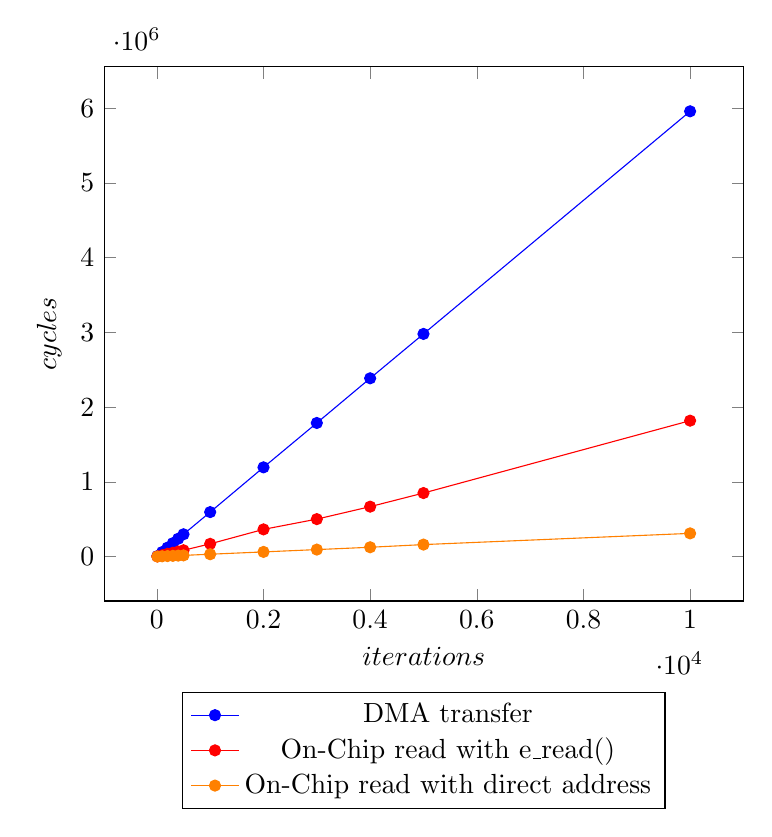
\begin{tikzpicture}
	\begin{axis}[
        xlabel=$iterations$,
        ylabel=$cycles$,
        legend style={at={(0.5,-0.17)},anchor=north},
        %xmode=log,
        %log basis x={10}
        width=0.8\textwidth
    ],
	\addplot[mark=*,blue] plot coordinates {
        (10,6000)
        (100,60000)
        (200,119242)
        (300,178631)
        (400,238313)
        (500,298039)
        (1000,595043)
        (2000,1194041)
        (3000,1788042)
        (4000,2386040)
        (5000,2980040)
        (10000,5960049)
    };
    \addlegendentry{\gls{DMA} transfer}
	\addplot[mark=*,red] plot coordinates {
        (10,1700)
        (100,17000)
        (200,36618)
        (300,50417)
        (400,67227)
        (500,84041)
        (1000,170000)
        (2000,363745)
        (3000,500980)
        (4000,667895)
        (5000,850000)
        (10000,1818769)
    };
    \addlegendentry{On-Chip read with e\_read()}
	\addplot[mark=*,orange] plot coordinates {
        (10,359)
        (100,3500)
        (200,6273)
        (300,9379)
        (400,12471)
        (500,15647)
        (1000,31000)
        (2000,62079)
        (3000,93061)
        (4000,124292)
        (5000,160000)
        (10000,310079)
    };
    \addlegendentry{On-Chip read with direct address}
	\end{axis}
\end{tikzpicture}
\caption{Performance measures based on number of cycles executed for a given number of iterations transferring 8 bits of data}
\label{graph transfert}
\end{figure}

\begin{figure}[h!]
\centering
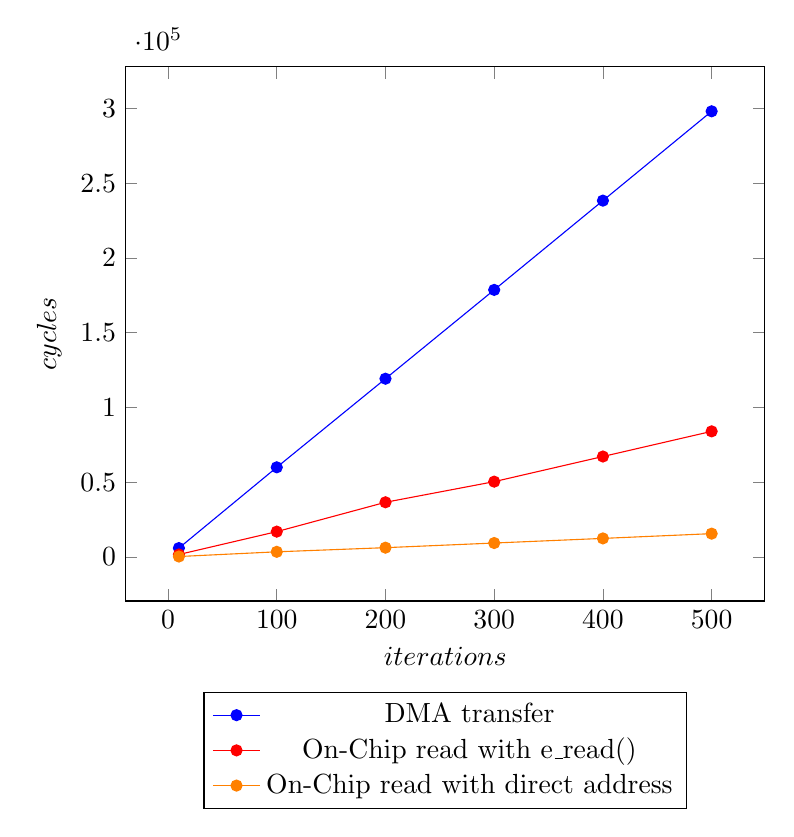
\begin{tikzpicture}
	\begin{axis}[
        xlabel=$iterations$,
        ylabel=$cycles$,
        legend style={at={(0.5,-0.17)},anchor=north},
        %xmode=log,
        %log basis x={10}
        width=0.8\textwidth
    ],
	\addplot[mark=*,blue] plot coordinates {
        (10,6000)
        (100,60000)
        (200,119242)
        (300,178631)
        (400,238313)
        (500,298039)
    };
    \addlegendentry{DMA transfer}
	\addplot[mark=*,red] plot coordinates {
        (10,1700)
        (100,17000)
        (200,36618)
        (300,50417)
        (400,67227)
        (500,84041)
    };
    \addlegendentry{On-Chip read with e\_read()}
	\addplot[mark=*,orange] plot coordinates {
        (10,359)
        (100,3500)
        (200,6273)
        (300,9379)
        (400,12471)
        (500,15647)
    };
    \addlegendentry{On-Chip read with direct address}
	\end{axis}
\end{tikzpicture}
\caption{Performance measures based on number of cycles executed for a given number of iterations transferring 8 bits of data, zoomed from 0 to 500 iterations}
\label{graph transfert2}
\end{figure}

It is important to note that we were only interested by measuring the transfer of a small amount of data. Using the \gls{DMA} is faster for bigger data size \cite{programmingadapteva}.


\section[Example 3]{Example: Transfer between host and eCores} \label{ex3}

Examples available on \href{https://github.com/nkcr/parallella-computing/tree/master/simple-epiphany/data-from-host-to-epiphany}{GitHub}\cite{githubproject}: \textit{simple-epiphany/data-from-host-to-epiphany}, \textit{simple-epiphany/data-from-host-to-eCore}.

The goal we want to reach is creating a shared space from the host, then filling it with data to be used by \glspl{eCore}.

Figure \ref{fig host to eCore} illustrates the process of how we will transfer data from the host to \glspl{eCore} (version a), or an individual \gls{eCore} (version b). We see that we can either use a shared memory buffer to set a memory available for every \glspl{eCore}, or we can directly write to an \gls{eCore}'s local memory. For the version \textit{a}, the steps are:

\begin{enumerate}
  \item[1a.] allocating the shared space (\code{e\_alloc}) from the host
  \item[2a.] filling the shared space (\code{e\_write}) from the host
  \item[3a.] loading \glspl{eCore} and make them use the shared space
\end{enumerate}

For the version \textit{b} the steps are simpler because we avoid the need of a shared memory buffer by directly writing to an \gls{eCore}'s local memory (\textit{1b}). Then, an \gls{eCore} can use it's local memory to read data set from the host (2b).

\begin{figure}[h!]
\centering
\includegraphics[width=0.7\textwidth]{examples/host_to_eCores.pdf}
\caption{Simplistic scheme of transferring data the host to \glspl{eCore}, or an individual \gls{eCore}}
\label{fig host to eCore}
\end{figure}

In this example, we will use 2 int arrays of 200 plus an array to store a result. Allocating memory and filling a shared buffer is not a tough task once we know how to use \code{e\_alloc} and \code{e\_write}. In the following code, we show the allocating and writing part:

\begin{lstlisting}
  e_mem_t shared_result;
  e_mem_t shared_x;
  e_mem_t shared_y;
  
  e_alloc(&shared_result, BUFOFFSET, ncores*sizeof(float));
  e_alloc(&shared_x, BUFOFFSET + ncores*sizeof(float), 
                                 200*sizeof(float));
  e_alloc(&shared_y, BUFOFFSET + ncores*sizeof(float) 
                               + 200*sizeof(float), 
                                 200*sizeof(float));
  
  float y[200];
  float x[200];
  for(i=0; i<200; i++) y[i] = x[i] = i;
  int status = e_write(&shared_x, 0, 0, 0x0, y, 
                       200*sizeof(float));
  printf("Status of shared_x writing: %i\n", status);
  status = e_write(&shared_y, 0, 0, 0x0, x, 
                   200*sizeof(float));
  printf("Status of shared_y writing: %i\n", status);
\end{lstlisting}

To get those buffers from the \gls{eCore}, one has just to set pointers to the right addresses. Getting the right addresses implies that we know exactly where memory is mapped. As seen in the first part of this document (section \ref{memory}), the linker description file (\gls{LDF}) gives us that information. In our case, shared memory starts at \code{0x8f00'0000}. Hence, we get our buffers starting with this base address plus an offset, corresponding each time to the cumulated size of the previous buffers. The following code shows the part on the \glspl{eCore}' source code where buffers are retrieved by setting pointers to corresponding addresses:

\begin{lstlisting}
  volatile float *result;
  volatile float *shared_x;
  volatile float *shared_y;
  
  result   = (volatile float *) (0x8f000000 + 0x4*num);
  shared_x = (volatile float *) (0x8f000000 + 16*sizeof(float));
  shared_y = (volatile float *) (0x8f000000 + 16*sizeof(float) 
                                            + 200*sizeof(float));
\end{lstlisting}

We can then use those buffers. In the following example, we read values from the x and y arrays then write a result to the result buffer. That result will tell us if the process successfully worked, because we will be able to read it from the host part:

\begin{lstlisting}
	*result = shared_matrix1[num] + shared_matrix2[num] 
	                              + num / 10.0;
\end{lstlisting}

Another way to write data from the host to the \gls{epiphany} is directly writing to an \gls{eCore}'s local memory. That method also uses the \code{e\_write} method. But, instead of giving as first parameter a shared\_buffer, we pass an \code{epiphany\_t} object, which represents a workgroup of \glspl{eCore} (see section \ref{workgroup}). We can then specify the \gls{eCore}'s coordinates, relative to the workgroup. 

The following code shows how a data is directly sent to an \gls{eCore}'s local memory:

\begin{lstlisting}
// Here we can select which eCore to unlock (eCore(0;1) there)
int ok = 1;
e_write(&dev, 0, 1, 0x4000, &ok, sizeof(int));
\end{lstlisting}

We note that we gave \code{0x4000} as the offset memory. That value corresponds to the relative offset memory of the local \gls{eCore}'s memory. As seen previously in this document, each \gls{eCore} has 4 banks of memory, starting from \code{0x0000} to \code{0x7fff}. Giving an offset of \code{0x4000} will write the data to the second bank of memory (see table \ref{table:eCore}).

From the \gls{eCore}, to read the values set from the host, we had to set a variable at the correct address. To make it easier, we declared a char array and specified it's location to be on the second bank of local memory (hence starting at the address \code{0x4000}). We then used that array to place or read the data. The following code shows how we declared the array and how we placed the data:

\begin{lstlisting}
	volatile int instructions[8] SECTION(".text_bank2"); // 0x4000
	// instruction[0] is at 0x4000
	// instruction[1] is at 0x4004
	int result = instructions[0]; // Data from the host
\end{lstlisting}


\section{Benchmark} \label{benchmark}

The point of this part is to implement the linpack benchmark test.Taking the existing c implementation, we will first simply run it only on the host part. We will then try to improve it by including the \gls{epiphany} in the process, using the \glspl{eCore}. We should be able to measure a better performance between the host only implementation and the one using the \gls{epiphany}.

The linpack works nearly out-of-the-box and only requires to adapt the \code{second} method, which is used to measure the performance. The result we obtained was approximately 120 MFlops, which is what we could expect from an ARM-A9 processor\cite{linpackpc}. We will now look at how we could include the \gls{epiphany} in the process.

Using linpack directly on the \gls{epiphany} won't work due to memory capacity (see figue \ref{code overflow}). What we will do is delegate jobs from the host to the \gls{epiphany}. To do so, we will set some data in the global memory, thus being available to the \glspl{eCore} and some status variables to know which \glspl{eCore} are already working or not. The host will have to poll each \glspl{eCore}' statuses, once it gets a free \gls{eCore} set to it some specific data required to compute and then tel the \gls{eCore} to do the work using global memory with it's specific data received from the host. Figure \ref{fig flow host} describes how the host part will interact. As long as there is still some work to do (more iterations), the host will look for a free \gls{eCore}, give to it some instructions and then release it.

\begin{figure}[h!]
\begin{lstlisting}[language=bash]
... ld: clinpack.elf section `.bss' will not fit in region `INTERNAL_RAM'
... ld: region `INTERNAL_RAM' overflowed by 318544 bytes
\end{lstlisting}
\caption{Memory capacity exceeded if using c linpack on the \gls{epiphany}}
\label{code overflow}
\end{figure}

\begin{figure}[h!]
\centering
\includegraphics[width=1\textwidth]{flow_linpack_host.png}
\caption{Activity diagram on the host side}
\label{fig flow host}
\end{figure}

On the \gls{epiphany} part (see figure \ref{fig flow epiphany}), each \gls{eCore} waits to be released by the host, compute what is needed using global data and specific ones (instructions), write the result and loops again. It is stopped only when application exits.

\begin{figure}[h!]
\centering
\includegraphics[width=1\textwidth]{flow_linpack_epiphany.png}
\caption{Activity diagram on the \gls{epiphany} side}
\label{fig flow epiphany}
\end{figure}

Using that process works for a small number of iterations. We implemented the concept inside a loop called once. But no relevant changes were observed since the section optimized did not represent a significant part of the benchmark. We had the same performance.

When profiling the linpack implementation (using \code{gprof}), we found out that approximately 88\% of the total running time spent by the benchmark is in one function (see figure \ref{code profilling}). That function (\code{daxpy}) makes the addition of an array plus an array multiplied by a constant. A more precise measure (using \code{gcov}), to see where the critical section is, showed us that the most used line within that function is called 69'679'500 times (see figure \ref{code profilling2}). So we will be focusing on optimizing this particular part of the code, which is the following code:

\begin{lstlisting}
for (i = 0;i < n; i++) {
  dy[i] = dy[i] + da*dx[i];
}
\end{lstlisting}

\begin{figure}[h!]
\begin{lstlisting}
Flat profile:

Each sample counts as 0.01 seconds.
  %   cumulative   self              self     total           
 time   seconds   seconds    calls  us/call  us/call  name    
 88.49      1.23     1.23  1060694     1.16     1.16  daxpy
  7.91      1.34     0.11                             matgen
  2.88      1.38     0.04                             dgefa
  0.72      1.39     0.01    20394     0.49     0.49  dscal
  0.00      1.39     0.00    20394     0.00     0.00  idamax
  
\end{lstlisting}
\caption{Results of the c linpack profilling using gprof}
\label{code profilling}
\end{figure}

\begin{figure}[h!]
\begin{lstlisting}
 69679500:  572:        for (i = 0;i < n; i++) {
 69679500:  573:                dy[i] = dy[i] + da*dx[i];
        -:  574:        }
\end{lstlisting}
\caption{c linpack Line profiling of the most used line using gcov}
\label{code profilling2}
\end{figure}

Using the process we described previously (fig \ref{fig flow host} and fig \ref{fig flow epiphany}), we faced a critical deadlock while executing the program. After a while, all \glspl{eCore} were in a busy state and didn't change their state ever. 

Trying to solve the problem, we saw that it never happened after the same number of iterations. To get a better idea of what could cause the deadlock, we made a merged activity diagram showing data access (figure \ref{fig flow general}). It seemed that status variable was read both at the same time by the \gls{epiphany} and the host side, it could have been the source of our deadlock.

\begin{figure}[h!]
\centering
\noindent\makebox[\textwidth]{\includegraphics[width=1.4\textwidth]{flow_general.pdf}}
\caption{General activity diagram}
\label{fig flow general}
\end{figure}

From figure \ref{fig flow general}, we developed another activity diagram preventing the program accessing the same variable at the same time (figure \ref{fig flow general V2}). That way, we would use shared memory and local \glspl{eCore}' memory. It would prevent the host and \gls{epiphany} side polling the same variables at the same time.

\begin{figure}[h!]
\centering
\noindent\makebox[\textwidth]{\includegraphics[width=1.4\textwidth]{flow_general_V2.pdf}}
\caption{General activity diagram second version using \glspl{eCore}' local memory}
\label{fig flow general V2}
\end{figure}

\subsection{When hardware meets software}

Before implementing our second activity diagram (fig \ref{fig flow general V2}) and after some time testing some possibilities of what could cause our deadlock, we observed a curious fact: our program always took more time to come to a deadlock when it was used after a time of inactivity. It is shown in graph \ref{graph deadlock temp}. Based on this observation, we suspected temperature to be involved in our problem. After more precise measures, it came that temperature was definitely the cause of our deadlock. As shown in graph \ref{graph deadlock temp2}, above 69°C, system became instable and gave unpredictable results. Looking at adapteva's hardware github repos \cite{githubadaptevahard}, we found out that an issue warns us about the parallella becoming unstable under unless cooled properly\cite{githubadaptevahardissue}. This new factor will then be watched in our future implementation. Graph \ref{graph deadlock temp} and \ref{graph deadlock temp2} show number of iterations and temperature after and before a launch of our program. We measured temperature of the parallella, then we launched our program and measured temperature reached when deadlock occurred as well as number of iterations executed. It is not surprising to observe that if the parallella is cooler, number of iteration before deadlock increases accordingly (graph \ref{graph deadlock temp}). Deadlocks in our measures start from 69.2°C to 70.6°C (graph \ref{graph deadlock temp2}. Measuring a pertinent range of temperature was a tough task because, after each test, the parallella was at it's warmest. We had to cool the heatsink, wait, or use a fan. In some cases, the parallella could have been harder to warm because we would have cooled the heatsink, thus taking more time and giving more iterations before coming to a deadlock.

Leaving from this observation, we will now be more careful to properly cool the parallella by adding a fan or placing it in a cooler area. We leave the final implementation of the linpack for the next chapter.

%\begin{tikzpicture}
%\begin{axis}[
%	title={Grids with shader=faceted interp}]
%
%\addplot3[patch,patch refines=3,
%		shader=faceted interp,
%		patch type=biquadratic]
%coordinates {
%	%(47.7,69.2,108788)
%	(66.1,69.6,1603)
%	(66.6,69.6,2902)
%	(66.6,70.6,1021)
%	(66.8,69.8,860)
%	(67.4,69.8,1399)
%	(66.9,69.5,364)
%	(66.9,70.1,1260)
%	(67.6,70.2,609)
%	(67.4,69.8,181)
%	
%	%(52.1,69.6,89814)
%	(66.0,69.6,2101)
%	(66.9,69.8,3291)
%	(67,70.6,1865)
%	(67.5,70,953)
%	(66.6,70.1,854)
%	(67.4,69.8,847)
%	(67.6,70,1025)
%	(67.4,69.7,164)
%	(67.5,69.8,1058)
%	
%	%(51.5,69.3,90775)
%	(65.8,69.8,2798)
%	(66.6,69.8,1699)
%	(66.3,69.6,645)
%	(67.3,70,804)
%	(66.9,70.2,1496)
%	(67.4,70.1,793)
%	(66.9,70.2,678)
%	(67.3,70.1,942)
%	(66.9,69.6,882)
%};
%\end{axis}
%\end{tikzpicture}

\begin{figure}
\centering
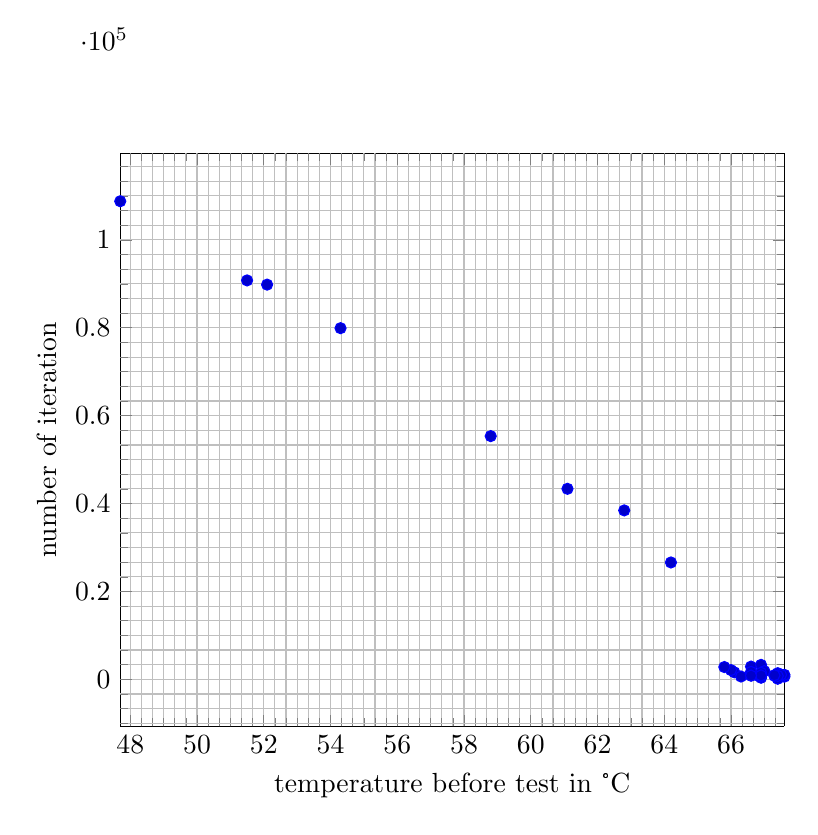
\begin{tikzpicture}
\begin{axis}[view={0}{0},
	grid=both,
	minor tick num=5,
	scale only axis,
	only marks,
	xlabel=temperature before test in °C,
	ylabel=temperature when blocked in °C,
	zlabel=number of iteration]
\addplot3+[] 
coordinates {
	(47.7,69.2,108788)
	(66.1,69.6,1603)
	(66.6,69.6,2902)
	(66.6,70.6,1021)
	(66.8,69.8,860)
	(67.4,69.8,1399)
	(66.9,69.5,364)
	(66.9,70.1,1260)
	(67.6,70.2,609)
	(67.4,69.8,181) % e
	(52.1,69.6,89814)
	(66.0,69.6,2101)
	(66.9,69.8,3291)
	(67,70.6,1865)
	(67.5,70,953)
	(66.6,70.1,854)
	(67.4,69.8,847)
	(67.6,70,1025)
	(67.4,69.7,164)
	(67.5,69.8,1058) % e
	(51.5,69.3,90775)
	(65.8,69.8,2798)
	(66.6,69.8,1699)
	(66.3,69.6,645)
	(67.3,70,804)
	(66.9,70.2,1496)
	(67.4,70.1,793)
	(66.9,70.2,678)
	(67.3,70.1,942)
	(66.9,69.6,882) % e
	(61.1,69.3,43354)
	(58.8,69.3,55343)
	(54.3,70.2,79905)
	(64.2,70,26593)
	(62.8,70.3,38439) % repeat
	(66.6,70.1,854)
};

\end{axis}
\end{tikzpicture}
\caption{Temperature before test vs the number of iterations reached just before deadlock}
\label{graph deadlock temp}
\end{figure}

\begin{figure}
\centering
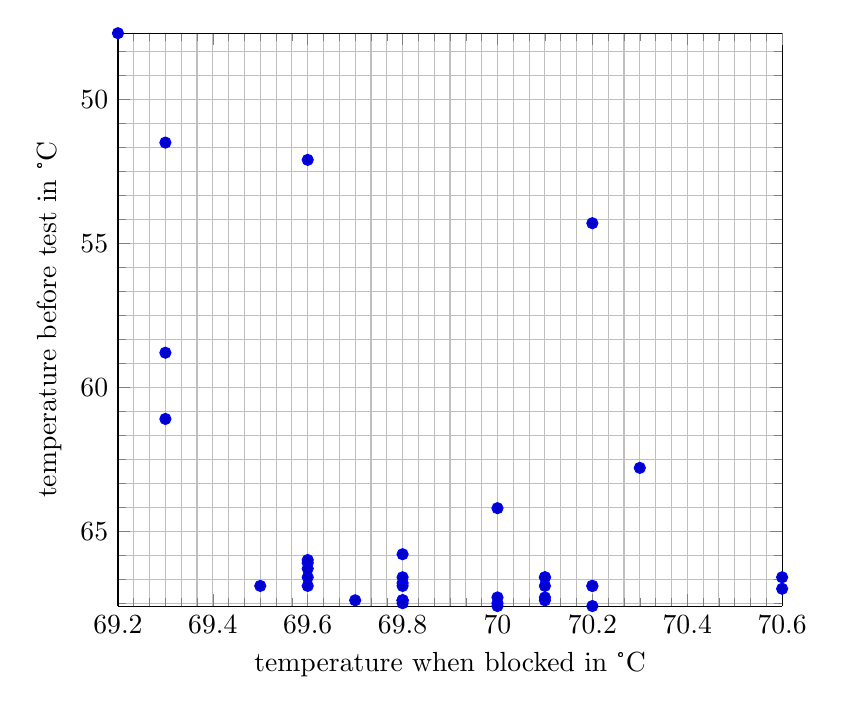
\begin{tikzpicture}
\begin{axis}[view={90}{90},
	grid=both,
	minor tick num=5,
	scale only axis,
	only marks,
	xlabel style={rotate=90},
	xlabel=temperature before test in °C,
	ylabel=temperature when blocked in °C,
	zlabel=number of iteration]
\addplot3+[] 
coordinates {
	(47.7,69.2,108788)
	(66.1,69.6,1603)
	(66.6,69.6,2902)
	(66.6,70.6,1021)
	(66.8,69.8,860)
	(67.4,69.8,1399)
	(66.9,69.5,364)
	(66.9,70.1,1260)
	(67.6,70.2,609)
	(67.4,69.8,181) % e
	(52.1,69.6,89814)
	(66.0,69.6,2101)
	(66.9,69.8,3291)
	(67,70.6,1865)
	(67.5,70,953)
	(66.6,70.1,854)
	(67.4,69.8,847)
	(67.6,70,1025)
	(67.4,69.7,164)
	(67.5,69.8,1058) % e
	(51.5,69.3,90775)
	(65.8,69.8,2798)
	(66.6,69.8,1699)
	(66.3,69.6,645)
	(67.3,70,804)
	(66.9,70.2,1496)
	(67.4,70.1,793)
	(66.9,70.2,678)
	(67.3,70.1,942)
	(66.9,69.6,882) % e
	(61.1,69.3,43354)
	(58.8,69.3,55343)
	(54.3,70.2,79905)
	(64.2,70,26593)
	(62.8,70.3,38439) % repeat
	(66.6,70.1,854)
};

\end{axis}
\end{tikzpicture}
\caption{Temperature reached when deadlock occurred along with temperature when started}
\label{graph deadlock temp2}
\end{figure}

%\begin{tikzpicture}
%\begin{axis}[
%    ybar,
%    enlargelimits=0.15,
%    legend style={at={(0.5,-0.15)},
%      anchor=north,legend columns=-1},
%    ylabel={\#participants},
%    symbolic x coords={m1,m2,m3},
%    xtick=data,
%    nodes near coords,
%    nodes near coords align={vertical},
%    ]
%\addplot coordinates {(m1,47.7)   (m2,66.1) (m3,66.6)  };
%\addplot coordinates {(m1,69.2)   (m2,69.6) (m3,69.6) };
%\addplot coordinates {(m1,108788) (m2,1603) (m3,2902) };
%\legend{used,understood,not understood}
%\end{axis}
%\end{tikzpicture}

\section{Conclusion}

We learnt in this chapter how to transfer data among the host and the \glspl{eCore}. If we understand well how memory is mapped and how the \glspl{SDK} provided by Adapteva work, it is not a tough task. Knowing how data transfers work is essential to start developing on the parallella, it will allow us to properly make \glspl{eCore} communicating among them and with the host. We also reached the physical limits of the parallella, either by trying to fit the linpack implementation on the \gls{epiphany}, reaching its memory limit, or by under cooling the parallella until it became instable. What we learnt from those examples and observations will be useful for the next chapter. Let's move to some practical examples.

\chapter{A practical example}
Moving from all we learnt in the previous chapters, this one will discuss the implementation of the linpack benchmark and the implementation of a $\pi$ approximation, using an easily parallelizable algorithm. It will be discussed the limits set by the granularity of a program and the speedup obtained with the \glspl{eCore} versus the host.

\section{Linpack}

The purpose of this section is to optimize the c linpack implementation with the help of the \gls{epiphany} side and its 16 cores. We will be optimizing a function computing a constant times a vector plus a vector :
\begin{lstlisting}
for (i = 0;i < n; i++) {
  dy[i] = dy[i] + da*dx[i];
}
\end{lstlisting}

We will attempt to take the model (see fig \ref{fig flow general}) discussed in the previous chapter and improve it, especially the \gls{epiphany} part. The aim is to beat 120MFlop obtained by the host part only.

The first results obtained with the help of the \gls{epiphany} side are much worse than those obtained with the host part only.

To communicate with the \gls{epiphany} side, we need to use shared buffer as shown in section \ref{ex3}. In our case - constant times a vector plus a vector - it implies declaring and using 3 shared buffers :

\begin{itemize}
  \item Vector[n], array of size n
  \item Vector[n], array of size n
  \item C, a constant
\end{itemize}

Those buffers are to be initialized each time the function is called :

\begin{lstlisting}
status = e_write(&shareddy,  0, 0, 0x0, dy, n*sizeof(REAL));
printf("[info] Status of shareddy writing: %i\n", status);
status = e_write(&sharedda, 0, 0, 0x0, &da,   sizeof(REAL));
printf("[info] Status of sharedda writing: %i\n", status);
status = e_write(&shareddx, 0, 0, 0x0, dx, n*sizeof(REAL));
printf("[info] Status of shareddx writing: %i\n", status);
\end{lstlisting}

Unfortunately for us, we measured that the only fact of initializing those buffers decreases performances by more than 5 times comparing to the host only implementation. Meaning that doing better than the host implementation is impossible with shared buffers. Figure \ref{graph flops decrease} shows metrics of KFlops measured with only the host side and with the buffer declaration.

As shown previously in figure \ref{code profilling}, the method we are working on is called 1060694 times. Hence, calling so often the buffers initialization is not reasonable and will never make better results than the host implementation. In a more general way, our program offers high concurrency and should have a coarse granularity to avoid excessive concurrency \cite{pie}. But the way we sent small operations to the \gls{epiphany} offers too much granularity by it's executing time and the number of time it is called comparing to the total executing time. Meaning that, in this particular case, transfer times are too important. In our case, we will not raise granularity since it would require changing the way linpack uses \code{daxpy}.

\begin{figure}[h!]
\centering
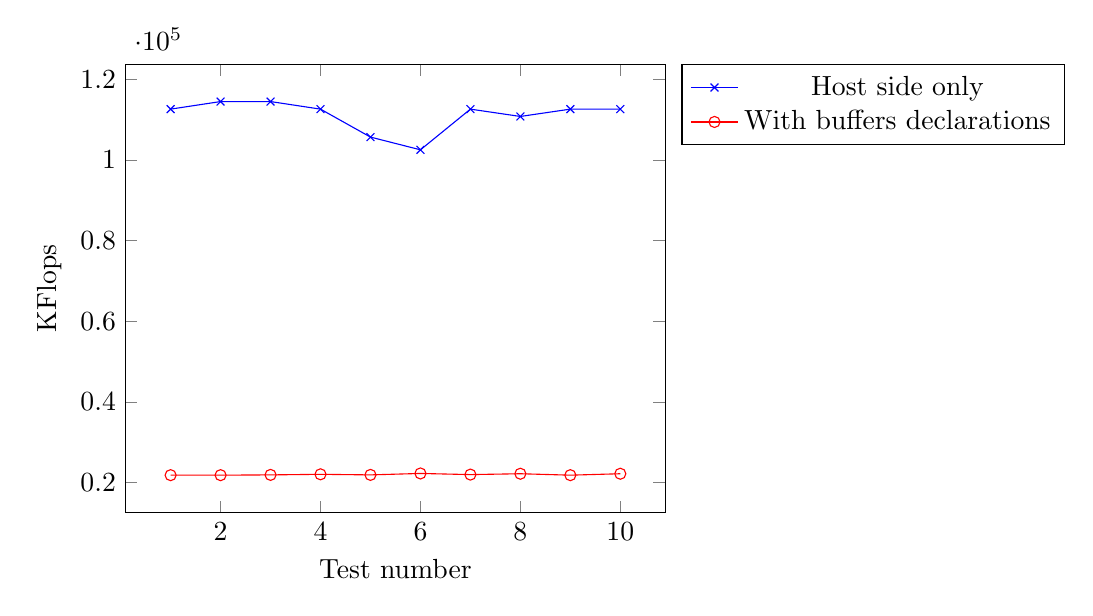
\begin{tikzpicture}
	\begin{axis}[
		xlabel=Test number,
		ylabel=KFlops,
		legend pos=outer north east]
	\addplot[color=blue,mark=x] coordinates {
		(1,112568)
		(2,114444)
		(3,114444)
		(4,112568)
		(5,105641)
		(6,102488)
		(7,112568)
		(8,110753)
		(9,112568)
		(10,112568)
	};
	\addlegendentry{Host side only}
	\addplot[color=red, mark=o] coordinates {
		(1,21868)
		(2,21868)
		(3,21938)
		(4,22079)
		(5,21938)
		(6,22294)
		(7,22009)
		(8,22222)
		(9,21868)
		(10,22222)
	};
	\addlegendentry{With buffers declarations}
	\end{axis}
\end{tikzpicture}
\caption{Measure of KFlops running c linpack on the host and with the shared buffers declaration. The host side is around 110MFlops, with shared buffer declaration arround 21MFlops.}
\label{graph flops decrease}
\end{figure}

Moving from this observation, we have three options :

\begin{itemize}
  \item Finding a way not to to initialize buffers in the function
  \item Finding a way not to use shared buffers
  \item Trying to raise the granularity by changing the implementation
\end{itemize}

Trying to initialize buffers outside the \code{daxpy} method is not possible since each time the method is called, we use new data to be shared. We could bypass the need of using shared buffers by exploiting the \glspl{eCore}' local memory, but this option would make the implementation more complex and be limited by the \glspl{eCore}' local memory size.

Finally, as said before, we would need to change the architecture of the linpack implementation to find a way of raising the granularity.

\section{$\pi$ approximation}

This section will be focused on implementing a concurrent program that will be approaching the PI value using machin-like formula (\ref{eq:machin-like}). The advantage of this formula is to be highly parallelizable. Because it is an infinite sum, we can easily distribute part of the sum across cores. 

\begin{equation}
	\pi = 4 \cdot \sum_{n=1}^{\infty} \frac{(-1)^n}{2n + 1}
	\label{eq:machin-like}
\end{equation}

We will be working on implementing an host only version of the PI approximation using machin-like formula, and an \gls{epiphany} version, using the \glspl{eCore}. The formula will be implemented as a loop calling a function which computes part of the sum. That function will then be distributed among \glspl{eCore}. The main loop size will represent the main number of iterations, and the part size of the sum the function will compute will be called the sub-iterations number.

Figure \ref{fig machin-like} is a representation of the sub and main iterations. The total number of iterations is given by the number of main iterations times the number of sub iterations. The sub iterations will be distributed among \glspl{eCore}.

\begin{figure}[h!]
\centering
\includegraphics[width=.5\textwidth]{machin-like.pdf}
\caption{Representation of the machin-like implementation using sub and main iterations}
\label{fig machin-like}
\end{figure}

The code remains simple, it is a loop calling $N$ times a function which runs $n$ iterations. Hence, it is computing the sum for $N \cdot n$ iterations. The code for the host only implementation is quite straightforward :

\begin{lstlisting}
for(i = 0; i < main_iteration; i++) {
  res = res + f(i);
}

float f(unsigned x) {
  float res = 0;
  unsigned a = x * sub_iteration;
  unsigned b = a + sub_iteration;
  for(; a < b; a++) {
    res += pow(-1,a) / (2*a + 1);
  }
  return res;
}
\end{lstlisting}

To adapt our code for the \gls{epiphany}, we moved the function computing the sub iterations to the \glspl{eCore}' program. We then made the host managing \glspl{eCore} to compute the sub iterations, getting results and making the addition of all \glspl{eCore} results. We used the same concept spoken in section \ref{benchmark}, but using only local \glspl{eCore}' memory to set instruction and getting results.

The first measures we made was comparing execution times between the host implementation and the \gls{epiphany} one. We also wanted to know the impact of the number of main iterations with respect to the number of sub iterations. What we did was executing our program inside two loops modifying the number of main and sub iterations. We did the same operations for the host only implementation and the \gls{epiphany} one. We then plotted the results in a 3D graph showing the main number of iterations, the sub number of iterations and the execution time.

Figures \ref{fig measures pi1} and \ref{fig measures pi2} show the 3D graph obtained after plotting our results. What we can note is that the variance of the main number of iterations and sub iterations for the same total number of iterations does not affect the execution time. Figure \ref{fig measures pi1} compares the two implementations, the host one is on top. We see that the \gls{epiphany} implementation is about two times faster. Figure \ref{fig measures pi3} gives a better representation of the performance, giving, for the two implementations, the total number of iteration with the execution time. Figure \ref{fig measures pi2} is the top view of the 3D graph for each implementations. We plotted on top of it curves showing values for $N*n$ (number of iterations times number of sub iterations is constant), showing that for the same number of iterations, the variance of $N$ and $n$ gives the same execution time.

\begin{figure}[h!]
\centering
\noindent\makebox[\textwidth]{\includegraphics[width=.8\textwidth]{measures/both.pdf}}
\caption{Comparing time execution of host only and \gls{epiphany} computation of pi using machin-like method}
\label{fig measures pi1}
\end{figure}

\begin{figure}
  \begin{subfigure}{.5\textwidth}
  \centering
  \noindent\makebox[\textwidth]{\includegraphics[width=1\linewidth]{measures/stats-archive-top.pdf}}
  \end{subfigure}
  \begin{subfigure}{.5\textwidth}
  \centering
  \noindent\makebox[\textwidth]{\includegraphics[width=1\linewidth]{measures/stats-archive-top.pdf}}
  \end{subfigure}
\caption{Top view of time execution with respect to iterations number}
\label{fig measures pi3}
\end{figure}

\begin{figure}[h!]
\centering
\noindent\makebox[\textwidth]{\includegraphics[width=.8\textwidth,page=2]{measures/both.pdf}}
\caption{Comparing time execution of host only and \gls{epiphany} computation of pi using machin-like method}
\label{fig measures pi2}
\end{figure}

Our second measure will be the speedup obtained by using the \gls{epiphany} comparing to using only the host with its ARM-A9 processor. For the test, we will need a constant number of iterations, $M$, which corresponds to $M = N \cdot n$ ($N$ is the number main of iterations, $n$ the number of sub iterations). To compute the speedup, we will run our program with different number of cores. Then, we will compare the execution time when using one core with the time obtained with one to sixteen cores (\glspl{eCore}).

To keep the same number of iterations, we will use those formulas :

\begin{align*}
	M = N \cdot n \\
	n = \frac{M}{k \cdot nb_{cores}}\\
	N = k \cdot nb_{cores}
\end{align*}

with $M$ the total number of iterations, $N$ the number of main iterations, $n$ the number of sub iterations, $nb_{cores}$ the number of cores and $k$ a factor dividing the number of sub iterations. In our measures, we chose a constant $M$ which is divisible by the total number of cores and a constant k. We then ran the program making the number of cores varying from 1 to 16 (the total number of \glspl{eCore}). With the time obtained, we used it to divide the reference time, taken as the time used by the host only (hence one core). This time is taken as the \textit{time to beat}.

Figure \ref{fig speedup} shows the speedup of the \gls{epiphany} according to the host. We see that to obtain the same performance of the host, we need to use seven \glspl{eCore} and the maximum speedup using all the \glspl{eCore} gives an execution time 2.24 times faster than the host only.

\begin{figure}[h!]
\centering
\noindent\makebox[\textwidth]{\includegraphics[width=.8\textwidth,page=1]{measures/speedup.pdf}}
\caption{Speed up results, the reference time is the host}
\label{fig speedup}
\end{figure}

In section \ref{architecture}, we saw that the host side runs an ARM-A9 at 866MHz, while each \gls{eCore} runs at 1GHz. So even using a single \gls{eCore} against the host should be faster, but our measures shows that a single \gls{eCore} is seven times slower than the host. In fact, the documentation provided by Adapteva\cite{epiphanyArch}\cite{parallellamanual} tells us that the 1GHz stands for the operating frequency of the \glspl{eCore}' mesh network. But, in out test, we didn't use that mesh network at all. Because each jobs was dispatched from the host to each individual \gls{eCore}, we didn't benefit from the mesh network provided by the \gls{epiphany} architecture. Hence, our results are reasonable given the fact that we didn't use all the capacities of the \gls{epiphany} architecture.

Taking a single \gls{eCore} as the reference time gives a linear growing speedup following nearly the ideal case. The figure \ref{fig speedup2} shows that our problem is well distributed among \glspl{eCore} and that the parallel portion of our program is near 100\%. In this case, transfer times are negligible. 

\begin{figure}[h!]
\centering
\noindent\makebox[\textwidth]{\includegraphics[width=.8\textwidth,page=2]{measures/speedup.pdf}}
\caption{Speed up results, the reference time is one \gls{eCore}}
\label{fig speedup2}
\end{figure}

%\begin{figure}[h!]
%\centering
%\noindent\makebox[\textwidth]{\includegraphics[width=.8\textwidth,page=3]{measures/speedup.pdf}}
%\caption{Efficiency based on speedup}
%\label{fig speedup}
%\end{figure}

\section{Conclusion}

In this chapter, we tried to improve the linpack implementation without any success. What we learnt from that was an important fact: concurrent programming cannot improve a program at a too small granularity level depending on its transfer times. In our case, communication times was far over the execution time of the code we wanted to improve. We would need to re-think the implementation of the linpack program so as to raise the granularity.

Moving from the linpack, we took this opportunity to implement an approximation of $\pi$ that would offer an easy concurrent implementation. We found out that, for this problem, the host is seven times faster than a single \gls{eCore}, and using sixteen \gls{eCore} against the host is only 2.24 times faster. That result is far bellow what we could expect. One explanation would be the way jobs are distributed, without using the \gls{epiphany} mesh network at all. The speedup taking a single \gls{eCore} as a reference time grows linearly, nearly following the ideal case. This show us that our problem is well distributed and communication times doesn't affect much the speed. It would have been interesting to test with more than sixteen cores, for example using many parallella boards connected together.

\chapter{Final thoughts}
\section{Conclusion}

We have seen an overview of the parallella architecture along with its main features, some practical examples and made some measures so as to study its potential. Although we didn't cover everything the parallella has to offer, we still can draw some conclusions.

The parallella is still in a growing stage. Released in 2012, it has not much evolved since today and there is still work to be done. Documentation and tools provided by Adapteva suffer from a lack of updates. What we missed the most was a way to debug program hosted on the \gls{epiphany}. Even performing a simple output print wasn't possible, which made testing and debugging harder. Another missing feature would be an interrupt line between the host and the \gls{epiphany} side. Without it, we were forced to use polling so as to fetch information and states of the \gls{epiphany} from the host.

The parallella is good only on specific cases. With its very limited memory and the cost of using shared memory, we saw that we couldn't adapt every concurrent program to the \gls{epiphany}. We had to consider the program size as well as the shared memory needed, as we saw it wasn't possible to adapt the clinpack implementation due to those restrictions. With the $\pi$ implementation, we saw that even with minimal transfers time, the program wasn't as fast as we would think. The reason was that the main advantage of the parallella is its mesh network of \glspl{eCore} providing high speed memory transfers, which we didn't use at all. Hence developing on the parallella asks sometimes to think differently so as to exploit all its potential.

With its low price and low electricity consumption, the parallella has certainly a place on the market of distributed system. But without a strong toolchain, easy workflow and serious documentation, it will be impossible for Adapteva to find its place and gain adoption in a larger scope than only experimented embed system users.

\section{Further work}

It would be interesting to adapt the $\pi$ implementation using the mesh network of \glspl{eCore}. The idea would be to send from the host all the job once in a single \gls{eCore}, and then make \glspl{eCore} capable of spreading jobs among them using the mesh network. It should be the best way to exploit the capacities of the parallella.

The parallella supports the Message Passing Interface (MPI), we didn't talk about it but it would certainly be worth exploring its potential on the parallella. For example by adapting the $\pi$ implementation with MPI.

Last but not least, one of the main requirement of the parallella is to be scalable to thousands of cores. There is much to do with setting up and developing on a distributed architecture using many parallellas, either connected using ethernet or using GPIO (General Purpose Input Output). We could then be able to measure the speedup with more than sixteen cores.

\printbibliography

\chapter*{Declaration of Authorship}
I hereby certify that the paper I am submitting is entirely my own original work except
where otherwise indicated. I am aware of the regulations concerning
plagiarism, including those regulations concerning disciplinary actions that may result
from plagiarism. Any use of the works of any other author, in any form, is properly
acknowledged at their point of use.

\bigskip
\bigskip

Place \hfil date \hfil signature

\appendix
\chapter{Source code structure}
Sources involved with this projet can all be found at: 

\begin{center}
	\code{https://github.com/nkcr/parallella-computing}
\end{center}

It contains three folders:

\textbf{Miscellaneous}: contains some tests to check deadlock on basic C operations. It was used to debug the linpack implementation.

\textbf{benchmark}: contains the clinpack implementation in few versions. One is the host only and the others (containing \textit{\gls{epiphany}} in their name) are the implementations for the \gls{epiphany}. There is also the $\pi$ approximation using machin-like formula in two versions, one for the host and the other for the \gls{epiphany}. Inside of them there is scripts to run measures which generate cvs files, there is also the measures used for this paper.

\textbf{simple-epiphany}: contains all the examples developed for the second chapter \textit{In Deep}. All the examples of memory transfers as well as a simple game of life reside in this folder.

Each folder contains a README file which describes the content of it. Please note that some code was used to produce simple technological test and may not be properly maintained, this it is not the case of the $\pi$ implementation.

\chapter{Versions used}
The distribution used for this project was:

\begin{lstlisting}
$ lsb_release -a
Distributor ID:	Linaro
Description:	Linaro 14.04
Release:	14.04
Codename:	trusty
\end{lstlisting}

Kernel release:

\begin{lstlisting}
$ uname -r
3.14.12-parallella-xilinx-g40a90c3
\end{lstlisting}

The parallella board was a desktop version with Zynq7010. All source code was plain ANSI C, compiled using gcc version 4.8.2. The \gls{epiphany} toolchain (\glspl{SDK}, e-gcc utility, ...) was of version version 4.8.2 20130729 (prerelease) (2015.1).

\end{document}

% https://www.sharelatex.com/blog/2013/08/02/thesis-series-pt1.html